\setcounter{chapter}{0} %this gives Chapter 1
\chapter{Introduction}
\label{chapter:introduction}

\setlength{\epigraphrule}{0pt}
\renewcommand{\epigraphflush}{center}
\setlength{\epigraphwidth}{11cm}
\epigraph{\textit{``[W]e choose to go to the moon [...] and do the other things, not because they are easy, but because they are hard...''}}{\textbf{John Fitzgerald Kennedy}}

Undoubtedly, we are living in an Age of Information, which is made possible by the advances in computer science. Miniaturisation has enabled the manufacture of increasingly powerful computers. As the individual components of such classical computers become smaller, they are nearing a regime where progress is complicated by quantum mechanical effects. Materials have unwanted behaviour when constructed in nanometre scale layers. Quantum tunnelling leads to current leaks, unreliable calculations, reduced power efficiency, and so on. Quantum mechanics, however, can be used to our advantage as well, allowing us to process information in previously unattainable ways. 

Richard Feynman \cite{Feynman1982,Feynman1986} proposed the idea of the universal quantum simulator, which is capable of simulating the physical behaviour of any quantum system. Since all computer operations are physical processes, this would be a universal computer as well. David Deutsch \cite{Deutsch1989} developed this idea into a set of requirements for a universal quantum computer. In his network model \cite{Deutsch1989}, the information is stored in two-state quantum systems (qubits) and the computer manipulates these qubits. It has been shown \cite{Barenco1995,Sleator1995} that it is sufficient to implement one- and two-qubit quantum gates for universal computation. The measurement of these qubits provides the output of the computing process.

Theoretical work in the field of quantum information processing showed that certain mathematical problems could be computed more efficiently in a quantum computer than in any classical computer. There are a number of such ``quantum algorithms''; important examples are Shor's factorizing algorithm \cite{Shor1994} and Grover's search algorithm \cite{Grover1997}. Both rely on entanglement to give a result much more quickly than classical computation.

Many different physical systems have been proposed for quantum information processing, including nuclear magnetic resonance (NMR) \cite{Nielson2000}, photons \cite{Knill2001}, Josephson junction circuits \cite{You2005}, quantum dots \cite{Engel2004}, trapped neutral atoms \cite{Briegel2000,Deutsch2000} and ions  \cite{Cirac1995, Cirac2000}.
NMR has been used to demonstrate small quantum algorithms, but faces great difficulty in scaling the system up to many qubits and operations. Photonic qubits deliver high fidelity single qubit operations and measurements, but implementing multi-qubit operations is challenging.
%cite!
Ion traps are among the most advanced of these technologies; indeed, all key functions of a quantum computer have already been demonstrated. 

Research groups with a good deal of experience with these techniques include NIST in Boulder, the Institute for Quantum Optics in Innsbruck, the University of Maryland\footnote{The group moved from the University of Michigan in 2007.}, the University of Oxford, the University of Aarhus, Denmark, the University of Barcelona and the University of Ulm. The landmark results in quantum computing experiments have so far emerged primarily from NIST, Innsbruck, Michigan and Oxford.

A Controlled-NOT gate proposed by J. I. Cirac and P. Zoller \cite{Cirac1995} was implemented by the NIST group \cite{Monroe1995} and the Innsbruck group \cite{Schmidt-Kaler2003}. It was followed by deterministic entanglement of four ions \cite{Sackett2000}, a controlled-phase gate with 97\% fidelity \cite{Leibfried2003a}, basic quantum error correction \cite{Chiaverini2004}, quantum state teleportation \cite{Riebe2004}, creation of a 6-qubit Schr\"odinger cat state \cite{Leibfried2005}, 8-qubit entanglement \cite{Haeffner2005}, ion-photon entanglement \cite{Blinov2004}, demonstration of the Deutsch-Jozsa algorithm \cite{Gulde2003}, a basic implementation of Grover's search \cite{Brickman2005}, and a simple quantum Fourier transform \cite{Chiaverini2005}. 

Ion trapping groups use different species of ions for their experiments. The most common ones are \ion{Be}{}, \ion{Mg}{}, \ion{Ca}{}, \ion{Cd}{}, \ion{Ba}{}, \ion{Yb}{} and \ion{Hg}{}. There is no obvious choice for ion species used in large scale ion trap arrays, and practical quantum information processors might even use a number of different species for different purposes (information storage, cooling, etc.). Some of the issues regarding this problem are covered in \cite{Steane1997,Ozeri2007}.


 In the Ion Trap Quantum Computing Group at the University of Oxford, \Ca{} ions are used. One of their advantages is that all relevant energy levels are addressable by diode lasers without frequency doubling, even including those in the neutral atom involved in the ionizing process, see Figure~\ref{fig:levels}. Experiments in Oxford included Schr\"odinger's cat states \cite{McDonnell2007}, deterministic entanglement of a pair of spin qubits \cite{Home2006}, long lived memory qubits with $T_{2} \gtsim 45\s$ \cite{Lucas2007}, qubit readout with 99.991(1)\% fidelity \cite{Myerson2008}, and sympathetic cooling with two different isotopes of \CaI{} \cite{Home2009}. These experiments were conducted in a linear Paul trap with a single trapping region. 

\begin{figure}[t]
\begin{center}
$\begin{array}{cccc}
\mbox{\bf (a)} & 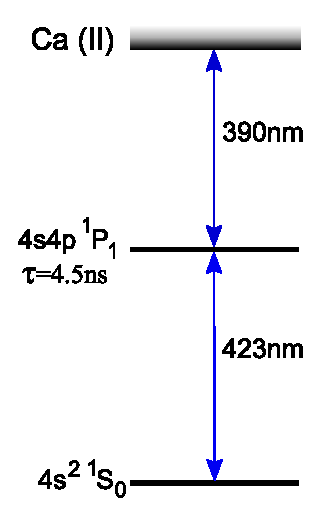
\includegraphics[width=4.2cm]{chapter1/levels/ca40atomlevels_v2} &
\mbox{\bf (b)} & \includegraphics[width=8.3cm]{chapter1/levels/ca40ionlevels_v3} \\
\end{array}$
\end{center}
\caption[Level structure of neutral \CaI{} and \Ca{}. ]{Level structure of (a) neutral \CaI{} and  (b) \Ca{}. The wavelength of the transitions are noted, as well as the level lifetimes and branching ratios in the case of \Ca{}. }
\label{fig:levels}
\end{figure} 


\section{The transition to microfabricated trap arrays}
\label{sec:transition}

The focus of research is now placed on more sophisticated trap designs, to allow larger scale information processing with large numbers of ions. The present thesis represents a contribution to this research.

The most popular approach is to use an array of ion traps with the ions being moved between the different trapping regions. Other ideas include using photonic qubits to couple together ion qubits at separate trapping regions, or using a large array of ions in a single trap.

The issue is now how to build multiple trap arrays. This approach of scaling up is being tackled by different research groups with a number of prototype traps. However there is no consensus about the ideal trap design and ion confinement in such trap arrays is in itself a major achievement. Surface traps \cite{Seidelin2006}, two \cite{Stick2006} and three layer \cite{Hensinger2006} structures are competing in terms of ease of manufacturing, trap stability, trapping strength, electric field noise and ease of optical access. 
%The first successful loading of ions in a microfabricated trap was reported in 2006 \cite{?}. Ion loading and experiments in a planar trap design from Sandia National Laboratories are presented in Chapters~\ref{chapter:apparatus}-\ref{chapter:heating}. These experiments took place slightly more than a year after the first success reported by the Maryland group and required building a completely new optical system, vacuum system, electronics and extending the experimental control software. A trap with three level structure from the University of Liverpool is also described theoretically in Chapter~\ref{chapter:simulation}.
%
%Methods of shuttling ions \cite{?} as well as separating and joining pairs of ions \cite{?} were also tested in certain traps. However, increased reliability and lower decoherence of the qubits during the procedures are necessary for useful quantum computing. The present work includes some theoretical analysis of this issue, and an experimental demonstration.
Methods of shuttling ions \cite{Hensinger2006,Huber2008} as well as splitting and joining pairs of ions \cite{Hensinger2006} in such traps are also an important area of investigation. The first successful loading of ions in a microfabricated trap was reported in 2006 by the Michigan \cite{Stick2006} and NIST groups \cite{Seidelin2006}. It was recognised in the ``Scientific American 50'' awards for 2006.
 
The work presented in this thesis has two major parts: computer modelling and theoretical description of segmented ion traps and their operation, and experimental evaluation of one microfabricated segmented ion trap. A completely new optical, electronic and vacuum apparatus was built to facilitate this and further studies of novel traps. A microfabricated trap array (electrode size of order 10\um) was built at Sandia National Laboratories, with design input from an international team including our group. Ion loading and experiments in this trap
are presented in Chapters~\ref{chapter:apparatus}-\ref{chapter:heating}. This was the first observation of ions in a microfabricated trap outside the USA.
 
A trap with an unusual three-layer geometry, designed for fast ion separation, is also modelled theoretically in Chapter~\ref{chapter:simulation}, and issues relevant to its operation are explored. The trap itself has subsequently  been successfully commissioned and use to trap ions.
 
The other theoretical studies presented in this thesis concern the issues of loading ions into small, shallow traps, and transporting ions through trap arrays with high speed and low heating. The former helped us to optimise the parameters for loading the Sandia trap, and should prove similarly helpful in future work with small traps. The latter introduces a method to allow the exact transport function of the potential well to be calculated, to make the ion follow a desired trajectory. This improves on previous treatments where transport functions were identified by trial and error or optimized imperfectly. A modest experimental demonstration was achieved by shuttling ions through the Sandia trap array.


\section{Thesis layout}
\label{sec:layout}

The first two chapters contain the theoretical topics of the thesis. Chapter~\ref{chapter:simulation} presents our computer modeling of ion traps, in particularly a mesoscopic segmented ion trap designed for fast ion separation and constructed by the University of Liverpool. The trap's behaviour is studied and the effect of micromotion and of manufacturing imperfections is explored. A microfabricated segmented ion trap design (prepared by Sandia National Laboratories, USA) is also introduced and modelled. 

Chapter~\ref{chapter:waveforms} contains theoretical calculations of two topics concerning ion traps. The first is the reliable, fast transport of ions with low heating. The second is a numerical simulation study of ion loading in the Sandia trap, performed to understand voltage and atomic beam requirements for successful ion trapping.

The subsequent four chapters contain the description of experiments with the Sandia trap. Chapter~\ref{chapter:apparatus} introduces the experimental setup: the vacuum system, the laser system, the optical layouts. Since the experiment was built up from scratch, the chapter includes observations of several issues encountered, including unusual laser modes, the stability of polarisation and the effect of the air conditioning system. Chapter~\ref{chapter:firstobs} describes the preparation of the vacuum system as well as the first observation of neutral atom fluorescence in the Sandia trap. The neutral atom density in the trap  and thus the calcium oven temperature is deduced. Chapter~\ref{chapter:sandia} describes details of a number of experiments to characterize the behaviour of the Sandia trap. Ion loading, micromotion compensation, ion lifetime estimation, trap frequency measurements and multiple ion loading are presented. Chapter~\ref{chapter:heating} first describes the characterization of the Doppler-cooling beams, which is important for the experiments to measure the heating rate of the ion trap. Heating rate measurements are then presented using time-resolved fluorescence during Doppler-cooling of ions. Finally, experiments implementing single ion shuttling in the Sandia trap are presented. Chapter~\ref{chapter:conclusion} gives a summary and conclusion.

